\makeheading{2019年度诺贝尔奖揭晓}\vskip1.5em
\greyboxNID{
\begin{minipage}{0.3\linewidth}
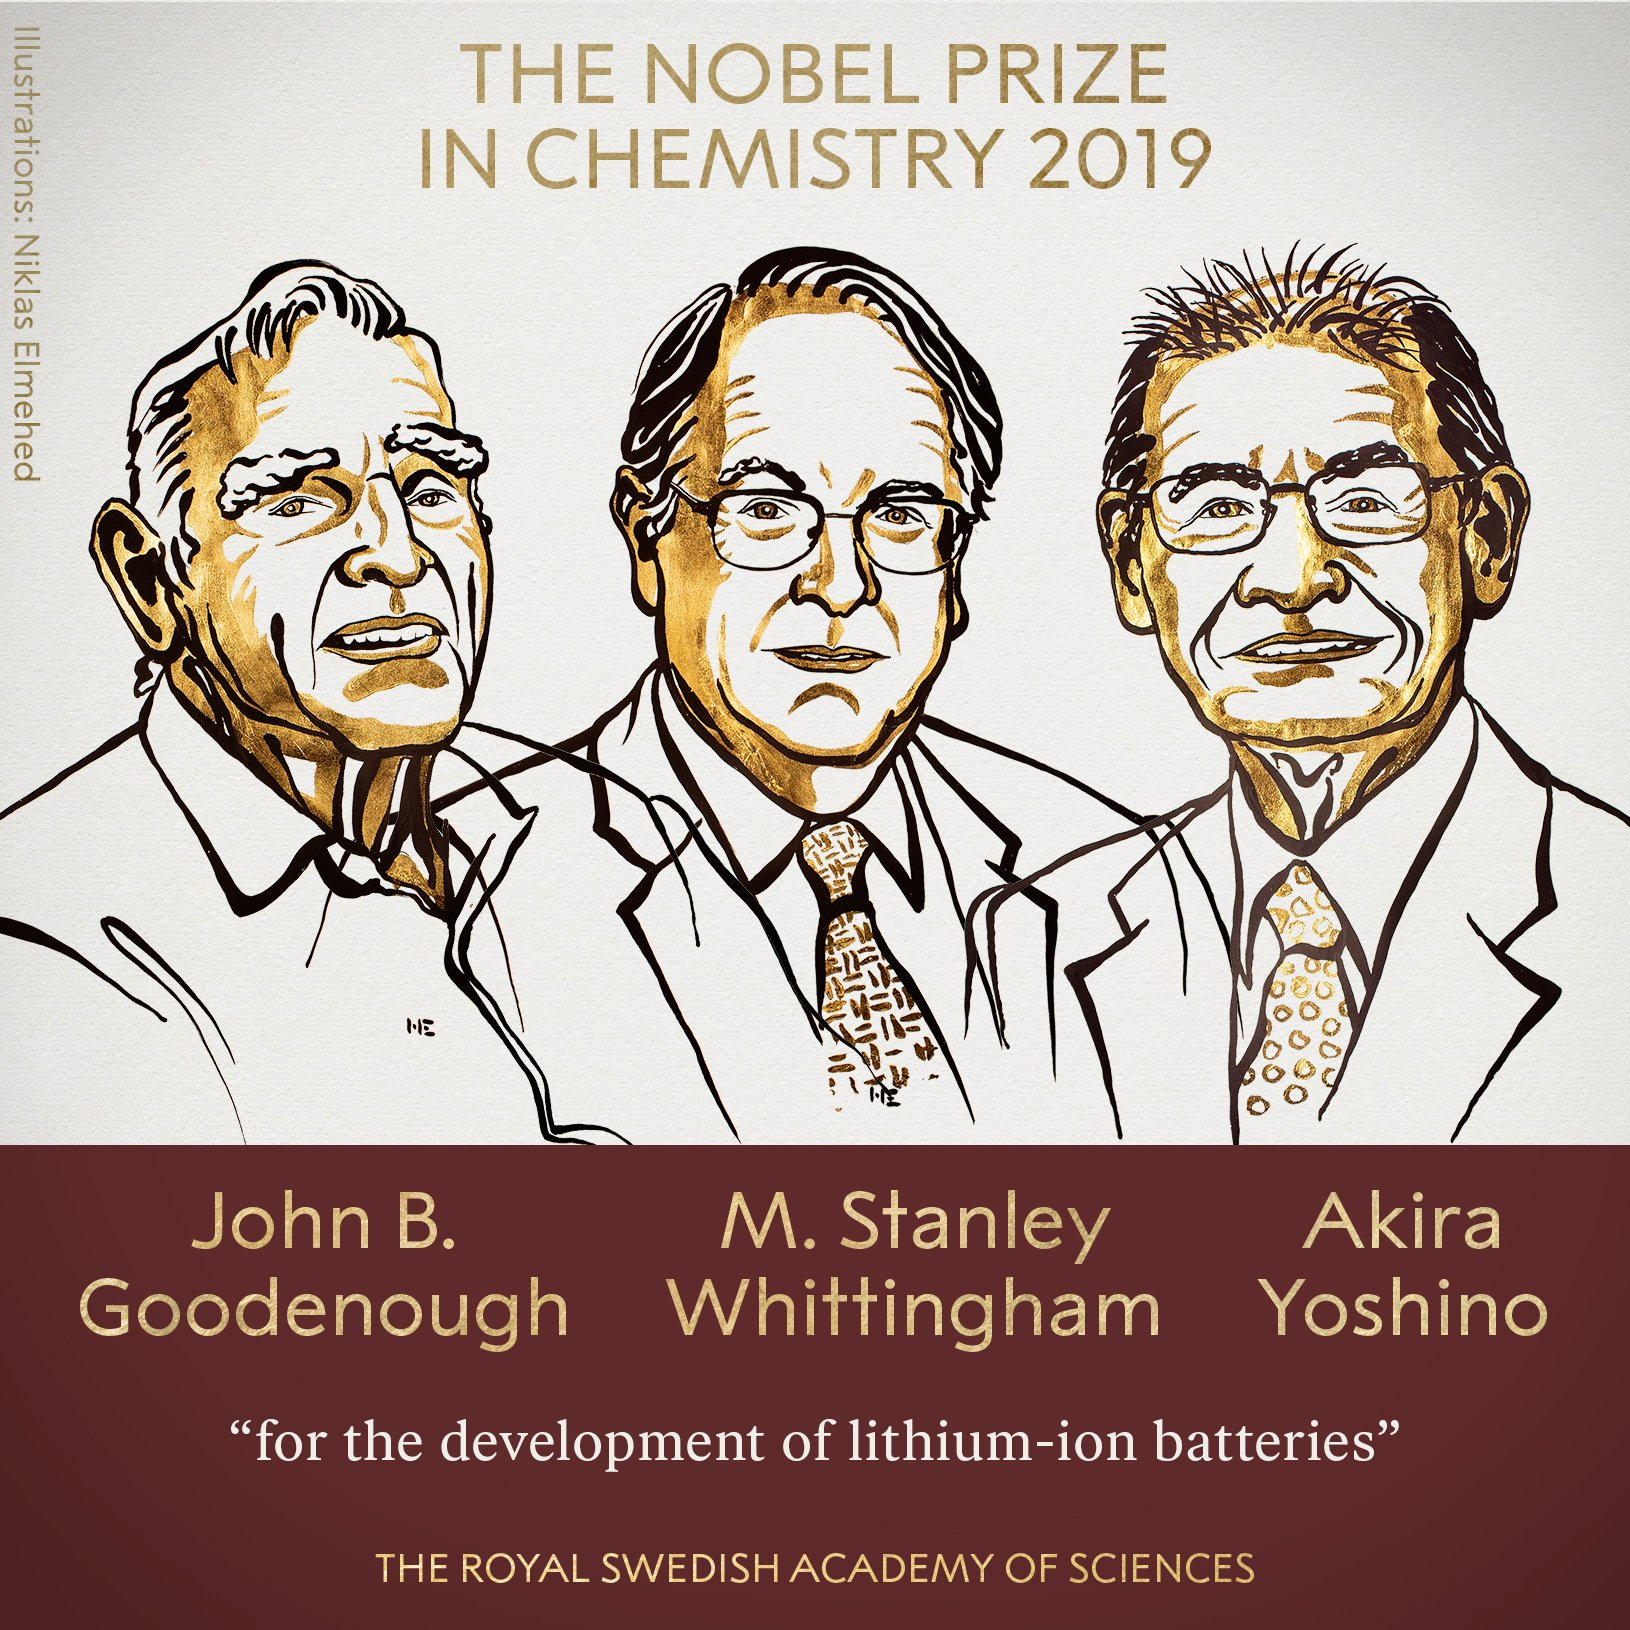
\includegraphics[width=\linewidth]{IMG/201910/191001.jpg}
\end{minipage}\hfill
\begin{minipage}{0.68\linewidth}
\textbf{\textsf{\color{color1} 诺贝尔化学奖}}\hfill 约翰·B·古迪纳夫\ \ \ M·斯坦利·惠廷汉姆\ \ \ 吉野彰

{\it\mbox{}\hfill——在锂离子电池领域的研发工作}\vskip0.4em

{\it  诺贝尔化学奖委员会表示,三位科学家对这种轻便、可充电电池的开发做出了重要贡献,这些电池如今驱动着移动电话等便携式电子设备,让“零化石燃料的社会”成为了可能. 

  诺贝尔奖基金会称,惠廷汉姆在20世纪70年代初发明了第一块功能性锂电池,但是古迪纳夫在1980年使用钴酸锂作为锂离子电池的正极,使电池的电势翻了一番. 五年后,吉野彰以古迪纳夫的发明为基础,制造出了第一块具有商业可行性的锂离子电池. }

\end{minipage}
}\vfill

\greyboxNID{
\begin{minipage}{0.3\linewidth}
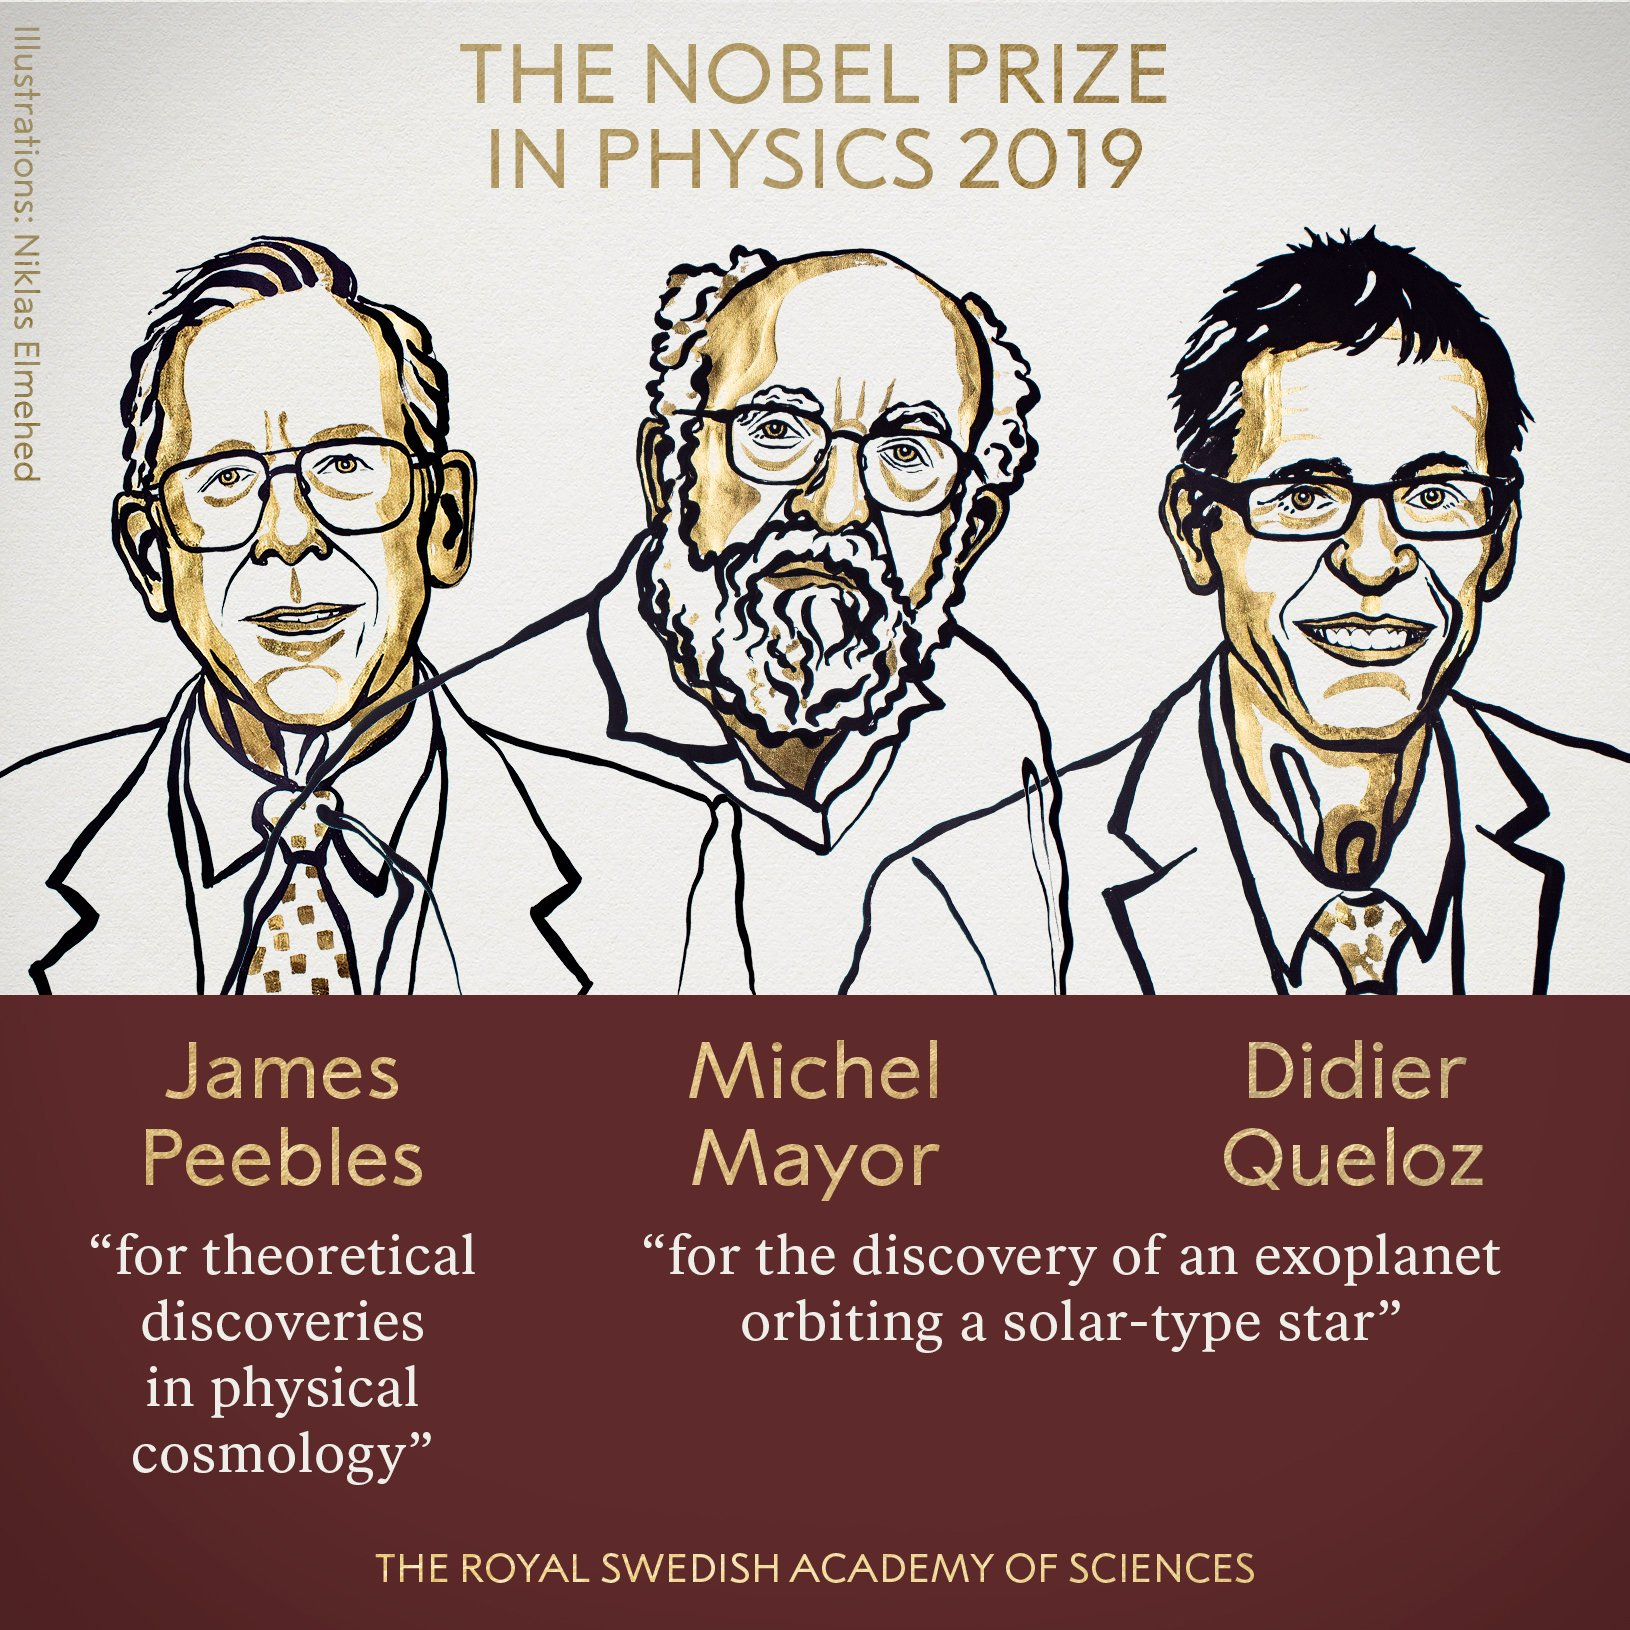
\includegraphics[width=\linewidth]{IMG/201910/191002.jpg}
\end{minipage}\hfill
\begin{minipage}{0.68\linewidth}
\textbf{\textsf{\color{color1} 诺贝尔物理学奖}}\hfill 吉姆·皮布尔斯\ \ \ 米歇尔·麦耶\ \ \ 迪迪埃·奎洛兹

{\it\mbox{}\hfill——在宇宙演化以及地外行星探索中的贡献}\vskip0.4em

{\it  1995年,日内瓦大学的麦耶和他当时的学生奎洛兹宣布发现了第一颗环绕类太阳恒星转动的太阳系外行星——开启了一个现在最热门的天文学领域. 他们通过这颗行星对飞马座51微小的引力探测到了这颗行星. 现在,人们仍然在使用这项技术研究已知的超过4000颗太阳系外行星. 

  皮布尔斯开发了一个理论框架. 诺贝尔奖委员会评论该框架构成了“现代理解从大爆炸一直到今天的宇宙历史的理论基础”. 
}

\end{minipage}
}\vfill

\greyboxNID{
\begin{minipage}{0.3\linewidth}

\includegraphics[width=\linewidth]{IMG/201910/191003.jpg}
\end{minipage}\hfill
\begin{minipage}{0.68\linewidth}
\textbf{\textsf{\color{color1} 诺贝尔生理学或医学奖}}\hfill 威廉·凯林\ \ \ 彼得·拉特克利夫\ \ \ 格雷格·塞门扎

{\it\mbox{}\hfill——在细胞如何通过调控基因开关感知并适应氧气变化上的发现}\vskip0.4em

{\it  动物需要氧气才能将食物转化成有用的能量,人们了解氧气的基础性重要作用已有数个世纪,但细胞如何适应氧气水平变化长期不为人知. 

  这一发现对于了解癌症和贫血等人类疾病非常重要. 他们的发现帮助研究人员更好地了解机体是如何适应低氧环境的——比如生成红细胞、长出新生血管等. 

  宾夕法尼亚大学的细胞生物学家Celeste Simon说:“他们所贡献的发现是根本性的,所有生物都离不开氧气,由此可见这项工作的意义. ”

}

\end{minipage}
}\vfill

\noindent\begin{minipage}{0.6\linewidth}

\greyboxNID{
\begin{minipage}{0.28\linewidth}\centering
    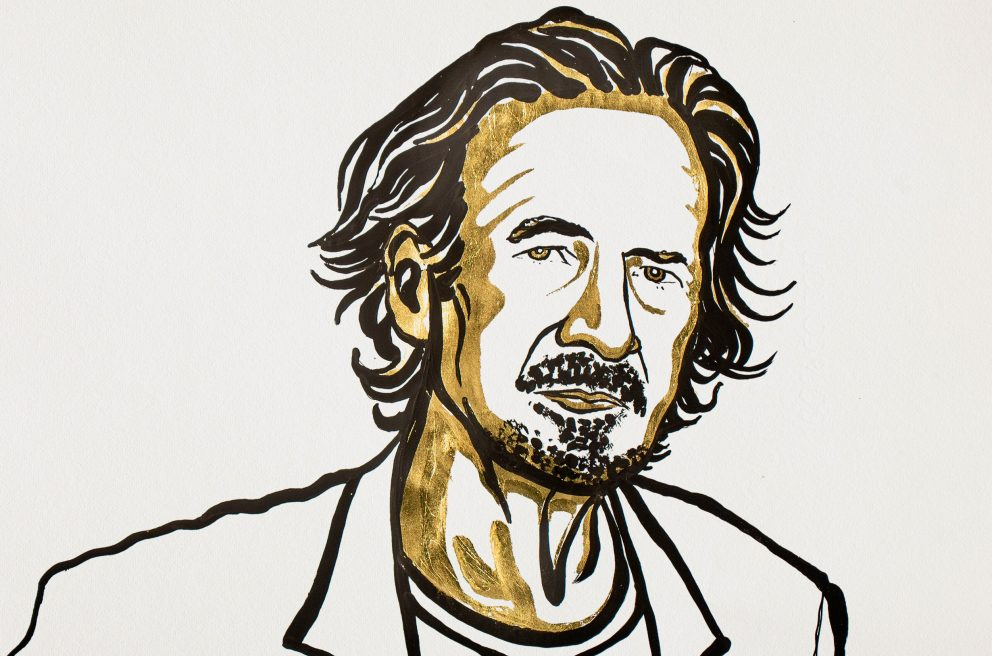
\includegraphics[width=0.7\linewidth]{IMG/201910/handke-3_2-992x656.jpg}\vskip1.8em
    
    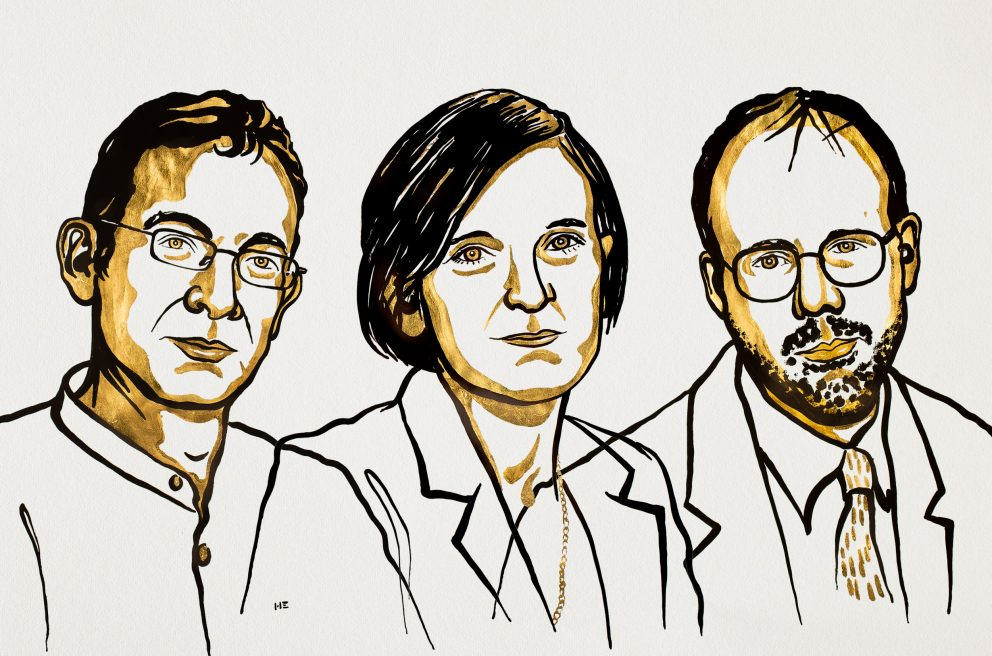
\includegraphics[width=\linewidth]{IMG/201910/eco-banerjee-duflo-kremer-3_2-992x656.jpg}\vskip1.8em
    
    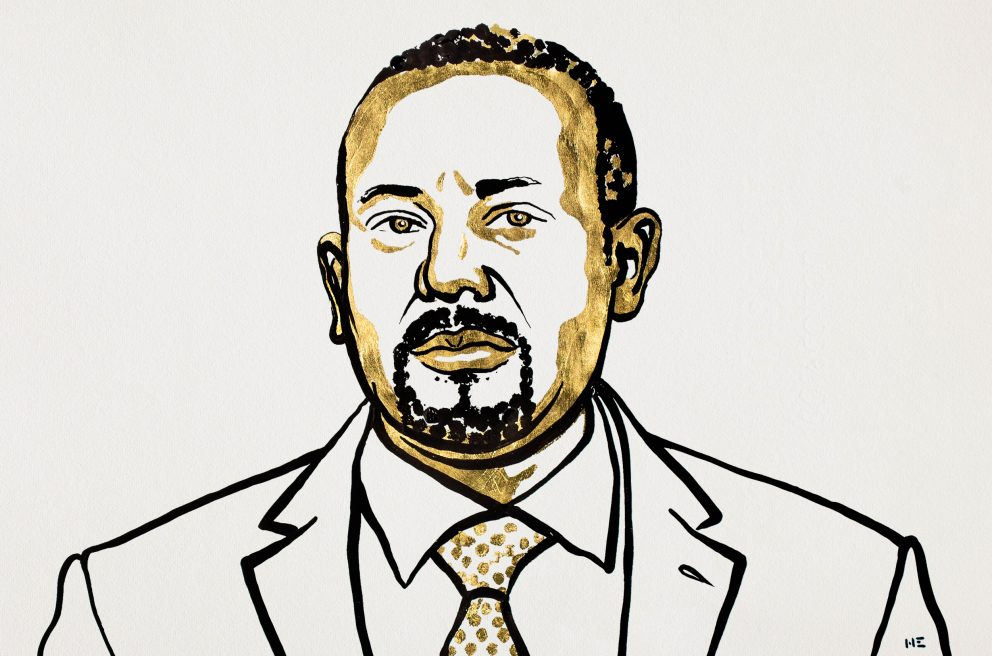
\includegraphics[width=0.7\linewidth]{IMG/201910/peace-ahmed-3_2-992x656.jpg}
\end{minipage}
\begin{minipage}{0.71\linewidth}
    \qiangdiao{诺贝尔文学奖}
    
    彼得·汉德克
    
    \textit{“用独创语言探索人类经验边界和特殊性”}
    
    \ 
    
    \qiangdiao{诺贝尔经济学奖}
    
    比吉特·班纳吉\ 艾丝特·杜芙若\ 迈克尔·克雷默
    
    \textit{“在减轻全球贫困方面的实验性做法”}
    
    \ 
    
    \qiangdiao{诺贝尔和平奖}
    
    阿比·艾哈迈德·阿里
    
    \textit{“在实现和平和国际合作所作出的努力”}
\end{minipage}
}
\end{minipage}\hfill
\begin{minipage}{0.37\linewidth}
    \greyboxNID{\vskip0.2em
        \begin{center}\vskip-0.5em
            {\large\qiangdiao{生活中的科学}}\vskip-1.5em
        \end{center}
        
        \begin{description}
            \item[Q1] \ 电脑黑色的壁纸会比白色的壁纸省电吗?
            \item[Q2] \ 超市里的扶梯是怎样卡住购物车的?
            \item[Q3] \ 为什么粥和牛奶在冷却时会在表面形成一层膜?
            \item[Q4] \ 为什么用手刮小票会有黑色纹路?
        \end{description}\vskip-0.3em
        
    }
\end{minipage}
\newpage
\makeheading{How we made the Li-ion rechargeable battery\\\vskip-0.5em
97岁“足够好”诺奖得主回忆锂离子电池研发之路}
\begin{center}
\greyboxNID{\centering\it
Progress in portable and ubiquitous electronics would not be possible without rechargeable batteries. 

如果没有可充电电池,无处不在的便携式电子设备将无法取得进步. 
}\vskip0.5em

    John B. Goodenough
    
    2018.03.09
\end{center}




\begin{multicols}{2}



A battery contains one or many identical cells. Each cell stores electric power as chemical energy in two electrodes, the anode and the cathode, which are separated by an electrolyte.

一个电池组包含一个或多个相同的小电池. 每个小电池将电能作为化学能存储在阳极和阴极之间,而两个电极被电解质隔开. 

The chemical reaction between the electrodes has an ionic and an electronic component. The electrolyte transports the ionic component inside a cell and forces the electronic component to traverse an external circuit. In a rechargeable battery, the chemical reaction is reversible. 

电极之间的化学反应具有离子和电子组分. 电解质在电池内部传输离子,并迫使电子穿过外部电路. 在可充电电池中,化学反应是可逆的. 

In the 1960s, chemists in Europe were exploring the chemistry of reversible insertion of lithium into layered transition-metal sulfides. At that time, rechargeable batteries used strongly acidic (\ce{H2SO4}) or alkaline (\ce{KOH}) aqueous electrolytes that offered fast hydrogen-ion (\ce{H+}) diffusion. The most stable cells used an alkaline electrolyte and a layered nickel oxyhydroxide (\ce{NiOOH}) as the cathode into which \ce{H+} is inserted reversibly to form the hydroxide \ce{Ni(OH)2}. However, an aqueous electrolyte limits the voltage of the cell and, therefore, the density of electric power a battery can deliver. 

20世纪60年代,欧洲的化学家们正在探索可逆地将锂插入层状过渡金属硫化物中的化学方法. 当时,可充电电池使用可使得氢离子(\ce{H+})快速扩散的强酸性(\ce{H2SO4})或强碱性(\ce{KOH})水性电解质. 最稳定的电池使用碱性电解质和层状羟基氧化镍(\ce{NiOOH})作为阴极,\ce{H+}可逆地插入其中以形成氢氧化物\ce{Ni(OH)2}. 但是,水性电解质限制了电池的电压,因此限制了电池可以传递的电能密度. 

In 1967, Joseph Kummer and Neill Weber of the Ford Motor Company discovered fast sodium-ion diffusion above 300°C in a ceramic electrolyte and invented a sodium–sulfur rechargeable battery that used the solid ceramic as the electrolyte, molten sodium as the anode and molten sulfur containing carbon felt as the cathode. The high operating temperature of above 300 °C made their battery commercially impractical, but it stimulated research into solid electrolytes and alternative battery strategies. At the time, I was working on transition-metal oxides at the MIT Lincoln Laboratory, and I was asked to monitor the development of this battery. The assignment introduced me to electrochemistry and to the challenge of developing a better oxide-based sodium-ion conductor.

1967年,Joseph Kummer 和 Neill Weber 发现在300°C以上的温度条件下,钠离子在陶瓷电解质中快速扩散,并发明了一种钠硫可充电电池. 该电池使用固体陶瓷作为电解质,熔融钠作为阳极,含硫的熔融碳作为阴极. 超过300°C的工作温度使其电池限制了其在商业上的可行性,但这一发明激发了对固体电解质和替代电池策略的研究. 当时,我在麻省理工学院林肯实验室从事过渡金属氧化物的研究,并承担监督该电池开发的任务. 这项任务使我进入了电化学领域,并面临着开发更好的基于氧化物的钠离子导体的挑战. 

In response, I developed, together with Henry Hong, an  electrolyte that had a framework structure and supported fast sodium ion conductivity; it was dubbed NASICON (NA SuperIonic Conductor) by colleagues after I left for the University of Oxford in 1976. 

作为回应,我与Henry Hong一起开发了一种电解质,该电解质具有骨架结构并支持快速的钠离子传导性.  1976年我离开牛津大学后,它被同事们称为NASICON(NA超离子导体). 

The oil crisis of the early 1970s exposed the vulnerability of US society, among others, to its dependence on imported oil and subsequently prompted investigations into solar and wind energy as potential sources for electric power. However, the intermittency of solar and wind meant that storage of this power would be required for these renewable sources to be useful. Hence, there was a desire for better rechargeable batteries. 

20世纪70年代初期的石油危机暴露了美国对进口石油的依赖这一脆弱性,随后促使人们开发了作为潜在能源的太阳能和风能. 但是,太阳能和风能的不稳定性意味着要使这些可再生能源发挥作用,就需要存储能量. 因此,存在对性能更强的可充电电池的进一步需求. 

Non-rechargeable batteries using a lithium anode and an organic-liquid electrolyte were known at the time, so the next step was to use the chemistry demonstrated in Europe of reversible lithium-ion insertion into transition-metal layered sulfide cathodes in order to create a rechargeable battery. Stanley Whittingham was hired by the Exxon Mobil Corporation to create such a rechargeable battery with a layered titanium disulfide (\ce{TiS2}) cathode that discharged to \ce{LiTiS2} through reversible lithium insertion. In 1976, Whittingham reported good initial performance for the cell. However, on repeated charging, plating of the lithium anode resulted to create an internal short circuit, which would ignite the flammable electrolyte. As a result, the program was abandoned a few years later. 

当时以锂离子作为阳极和有机液体作为电解质的不可充电电池已经问世,因此下一步工作是使用已在欧洲证明的可逆锂离子插入过渡金属层状硫化物阴极的化学方法,以制造出可充电电池. Stanley Whittingham(同为2019年诺贝尔化学奖得主)被埃克森美孚公司聘用以制造这种可充电电池. 该电池具有一个分层的二硫化钛(\ce{TiS2})阴极,该阴极通过可逆锂插入放电到 \ce{LiTiS2} .  1976年,Whittingham报告了该电池良好的初始性能. 然而,在重复充电时,却产生了会点燃可燃电解质的内部短路. 最终,该计划在几年后搁浅. 

Around this time, my group at the University of Oxford was investigating how much lithium can be extracted from a layered lithium cobalt oxide (\ce{LiCoO2}) or lithium nickel oxide (\ce{LiNiO2}) before the structure changed. I had reasoned that a rechargeable battery could be fabricated in a discharged, as well as a charged, state. We were able to demonstrate that over half of the lithium could be extracted reversibly with these cathode materials. This led Akira Yoshino to make the first lithium-ion rechargeable battery by combining the \ce{LiCoO2} cathode with a graphitic-carbon anode. This battery was used by the Sony Corporation to power the very first portable phone. 

大约在这个时候,我在牛津大学的研究小组正在研究在结构改变之前可以从层状钴酸锂(\ce{LiCoO2})或锂镍氧化物(\ce{LiNiO2})中提取多少锂. 我曾考虑过生产处于放电和充电状态的可充电电池. 我们能够证明这些正极材料可逆地提取一半以上的锂. 这引导了吉野彰(同为2019年诺贝尔化学奖得主)将\ce{LiNiO2}阴极与石墨碳阳极结合,并制造出第一款锂离子可充电电池. 索尼公司使用此电池为第一台手提电话供电. 

To lower the cost and increase safety, an all-solid-state rechargeable battery — where the liquid electrolyte is replaced with a solid electrolyte — is an active future direction for battery research. Indeed, rechargeable batteries with solid electrolytes are now being developed, including sodium batteries with a NASICON electrolyte. 

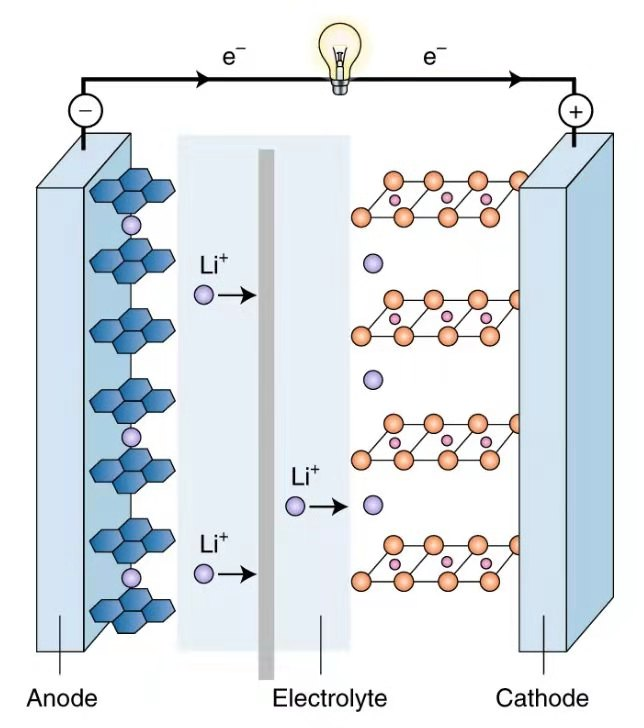
\includegraphics[width=0.8\linewidth]{IMG/201910/191004.jpeg}

为了降低成本并提高安全性,全固态可充电电池(用固态电解质代替液态电解质)是未来电池开发的积极可能方向. 事实上,研究人员正在开发具有固体电解质的可充电电池,包括具有NASICON电解质的钠电池. 

In 2015, a remarkable dielectric amorphous- oxide solid electrolyte was brought to me
by Maria Helena Braga of the University of Porto. It has lithium and sodium ion conductivities comparable to those of the organic-liquid electrolytes used in today’s lithium-ion batteries. At the University of Texas at Austin, where I moved to in 1986, we have used this unique solid to develop all-solid-state rechargeable batteries that are able to plate dendrite-free alkali-metal anodes with good contact over a long cycle life at acceptable charge and discharge rates. These developments suggest that all-solid- state batteries may soon be used to power all-electric road vehicles that are competitive with vehicles powered by fossil fuel in an internal combustion engine. 

2015年,波尔图大学的Maria Helena Braga给我的研究带来了理想的原料——电介质非晶体氧化物固体电解质. 它的锂和钠离子电导率可与当今锂离子电池中使用的有机液体电解质媲美. 1986年,我来到德克萨斯大学奥斯汀分校,并和同事们使用这种独特的固体来开发全固态可充电电池,该电池具有较长的使用年限和尚可接受的充放电速率. 这些技术进步表明,全固态电池可能将很快用于为电力汽车供电,并与化石燃料驱动内燃机车辆竞争. 

\mbox{}\hfill\textit{(全文有删减)}

\end{multicols}

\ADxinhangdao\vskip-4em

\makeheading{围绕另一颗太阳的第一颗行星}
\begin{center}
    \textit{2019 年诺贝尔物理学奖官方解读}
\end{center}

\begin{multicols}{2}
\greyboxNID{\qiangdiao{导读}

  人类是唯一孤独凝视着宇宙的物种么?在围绕另一个太阳的行星上,是否有生命存在?没有人知道. 但我们现在知道了太阳并不是唯一一颗有行星的恒星,在银河系中的数千亿颗恒星的绝大多数都有其伴随的行星. 天文学家现在已知超过 4,000 颗系外行星. }

Michel Mayor和Didier Queloz于 1995 年 10 月 在意大利佛罗伦萨举行的一次天文学会议上宣布了这一激动人心的发现. 这是第一颗被证明环绕类日型恒星运行的行星. 这颗被命名为飞马座51b的行星围绕飞马座51恒星飞速移动,其距离地球 50 光年,公转周期为 4 天(意味着其距离恒星很近,只有 800 万公里). 飞马座51恒星将该行星加热,温度超过1000℃. 由于地球距离太阳为1.5亿公里,公转轨道周期为1年,因此地球上温度要适宜很多. 新发现行星的体型大得令人惊讶——作为一个气态球体,其体积类似太阳系中的最大气态行星:木星. 

根据早期有关行星形成的理论,木星体型大小的行星应该在远离其恒星的位置产生,并且需要很长的公转周期. 木星环绕太阳的公转一周大约需要 12 年,因此天马座 51b 的 4 天短公转周期对寻找系外行星是个超级意外. 紧接着他们的发现,两个美国天文学家保罗·巴特勒和杰弗里·马西将他们的望远镜转向了天马座51b星系,然后确认了Mayor和Queloz的发现. 这些行星为什么距离恒星这么近?这个问题挑战着现有的有关行星起源的理论,并启发了新理论的提出. 新理论用来描述大的气体球在太阳系边缘被创造出来,随后向着其恒星旋进. 

\subsection*{完善方法,最终发现}

人们需要使用更为复杂的方案,才能追踪一颗系外行星. 所谓系外行星,是那些自己不会发光,只能靠反射来自其他星体的发出的光的行星. 一般这些光芒都被来自宿主恒星的耀眼光芒掩盖住了. 

 研究组用来发现系外行星的方法被称为\qiangdiao{径向速度法}(\textit{radial velocity method}). 宿主恒星在行星重力的影响下会发生移动,该方法由测量宿主恒星的移动来判定. 由于行星环绕恒星转动,恒星其实也在围绕着他们的共同质心发生转动. 在位于地球上的观测者看来,在视线方向上,这颗恒星看起来就像一会向后摇,一会向前摇. 而恒星的这种移动速度,也就是径向速度,可以通过广为人知的多普勒效应来进行测量. 多普勒效应说的是光线从一个移动物体上发出时,如果这个物体向着我们移动,光线会\qiangdiao{“变得更蓝”}(\textit{蓝移});而如果这个物体远离我们移动,光线会\qiangdiao{“变得更红”}(\textit{红移}). 这个效应其实和我们平时听到的救护车朝向我们开音调会变高,远离我们开音调会变低是一样的原理. 行星的这个效应使得恒星的光线选择性地变蓝或者变红. 天文学家用实验设备捕获的正是光波长的这些变化. 颜色上的变化可以通过恒星发出的光的波长精确测量,从而给出恒星在观察者的视线方向,也就是径向方向上的速度.  
 
径向速度特别小给这项研究带来了巨大的挑战. 举例来说,木星的引力使得我们的太阳绕着太阳系的质心以 12m/s 的速度运动,而地球的引力仅仅贡献了 0.09m/s . 发现类地行星对我们的仪器灵敏度提出了极高的要求. 为了提高精确度,天文学家同时测量数以千计的波长. 所有的光线利用光谱仪按照不同的波长区分开来,而这也正是这些测量的关键.     

\begin{figure}[H]
    \centering
    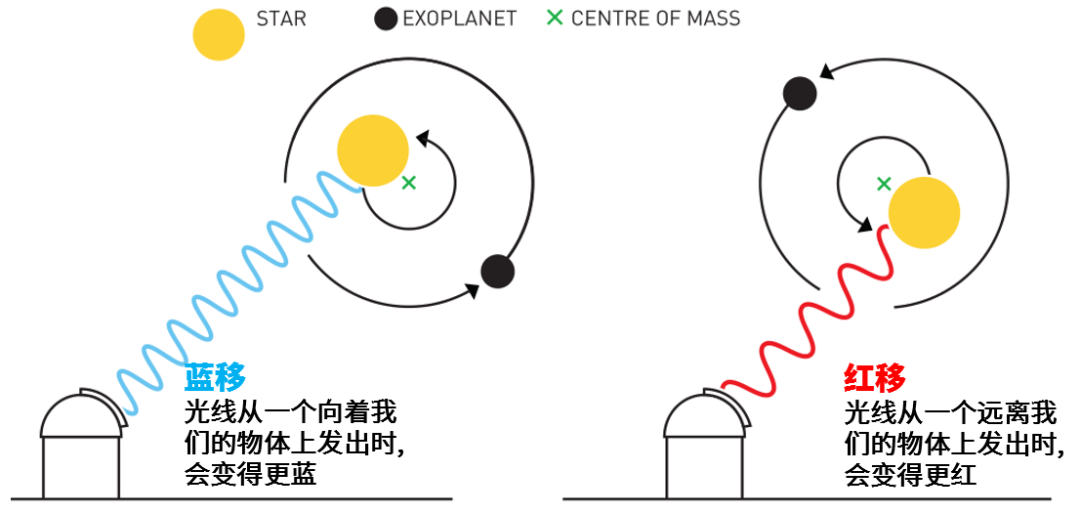
\includegraphics[width=0.8\linewidth]{IMG/201910/191005.png}
    \caption{\textit{恒星受行星引力的影响从而发生移动. 在地球上看来,恒星在视线方向上来回摆动. 这个运动的速度及其径向速度可以由多普勒效应确定,因为来自运动物体的光的颜色会发生变化. }}
\end{figure}\vskip-2em

\begin{figure}[H]
    \centering
    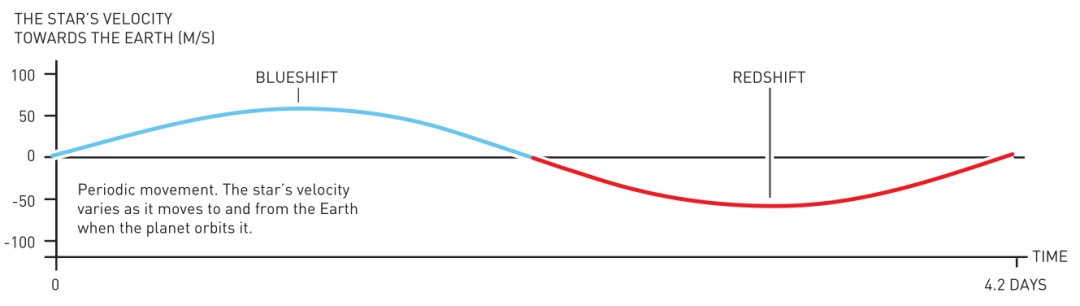
\includegraphics[width=0.8\linewidth]{IMG/201910/191006.png}
    \caption{\textit{恒星的周期性移动,使得径向速度发生周期性变化,从而出现周期性蓝移和红移. }}
\end{figure}\vskip-1em


20 世纪 90 年代早期,Queloz在日内瓦大学开始他的研究,Mayor已经花了很多年研究恒星运动,在其他研究人员的帮助下搭起了自己的测量仪器. 1977 年,Mayor在普罗旺斯天文台的望远镜上安装他早期的光谱仪. 这个仪器测量恒星速度的下限在 300 m/s 左右,而这个速度仍太大,以至于根本看不到有行星拖拽它的宿主恒星. Queloz与研究小组一起开发了新方法来进行更精确的测量. 他们利用了许多新技术,可以快速观察大量恒星并同时分析结果. 光纤可以将来自恒星的星光传送到光谱仪而不失真,更好的数字图像传感器(CCD)可以提高机器对光的灵敏度,功能更强大的计算机使得科学家能够开发用于处理数字图像和数据处理的定制软件. 当新的光谱仪于 1994 年春完工时,恒星运动的速度测量下限下降到 10 - 15 m/s,距离系外行星的发现已经非常接近了. 

\subsection*{更多的新世界等待揭晓}

围绕类太阳型恒星环绕的系外行星的首次发现开启了天文学的一场革命,上千万个未知的新世界呈现出来. 现在不仅可以通过地球上的望远镜,还可以通过卫星发现它们. 美国空间望远镜 TESS还可以扫描超过 20 万颗离我们最近的行星,并搜寻类似地球的行星. 之前,开普勒望远镜带来了许多丰硕的成果,其发现了超过 2300 个系外行星.  

随着径向速度的变化,现在寻找系外行星使用\qiangdiao{凌日法}. 它主要是测量一行星从恒星前方通过时,恒星光线强度的变化. 光会通过大气层传播,因此用凌日法还能观察到系外行星的大气层.  \vskip-1em

\begin{figure}[H]
    \centering
    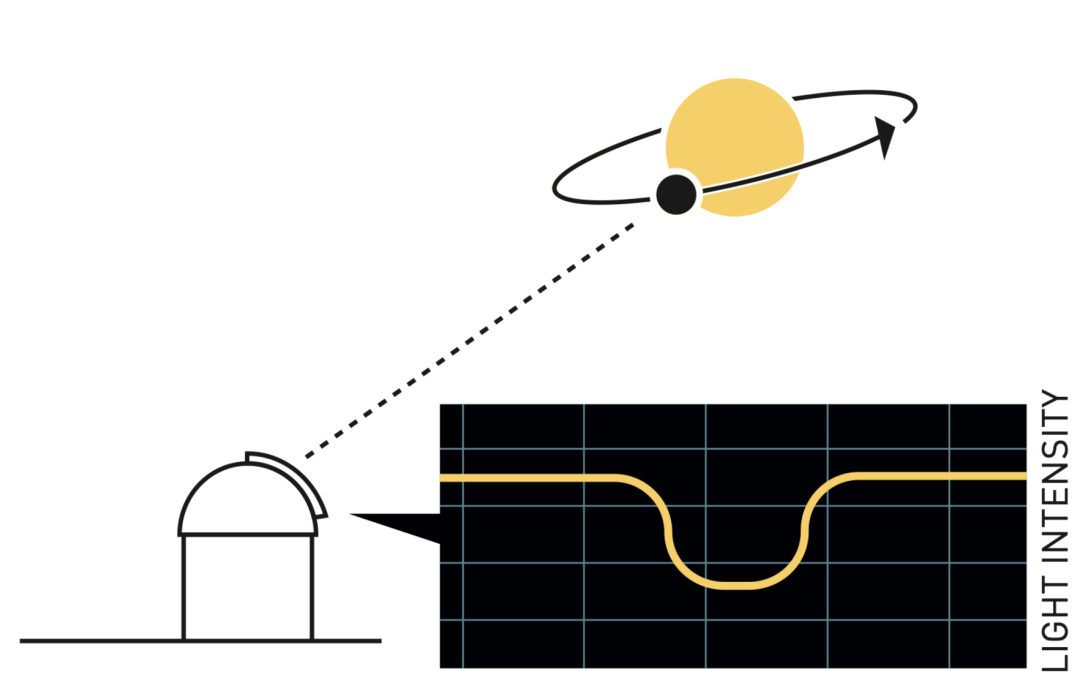
\includegraphics[width=0.8\linewidth]{IMG/201910/191007.png}
    \caption{\textit{当行星经过恒星和我们之间时,恒星的光强度会降低. 地球上的望远镜可以观察到这种影响. }}
\end{figure}\vskip-1em
     

迄今为止发现的系外行星以惊人的大小和轨道使我们感到惊讶. 它们挑战了我们先入为主的行星系统的观念,并促使研究人员修正了行星诞生的物理过程的理论. 随着众多寻找系外行星的项目开展,我们最终可能找到这个永恒的问题——宇宙中是否还有其他生命的答案.  

\end{multicols}
\vskip-0.5em

\qiangdiao{关于诺贝尔奖的更多信息,可在瑞典皇家科学院官网\url{www.kva.se/en/startsida}和诺贝尔奖官网\url{www.nobelprize.org}查阅. }\vskip-2em

\ADyixuehui\newpage

\makeheading{生活中的科学·上期答案}\vskip-1em

\begin{multicols}{2}

\noindent\qiangdiao{Q1为什么十五的月亮十六圆?}

民间之所以有“十五月亮十六圆”一说,是因为月球在椭圆轨道上绕地球转动,从一个满月到下一个,平均需要29天12小时44分. 在“望”时,月、地、日最接近一直线,月亮因此也最圆、最亮. 但由于月亮转速有快有慢,因此每次抵达“望”的时间不同,大多在每年的农历十六日甚至十七日凌晨. 

那么为什么月亮大多会在16日抵达“望”呢?

从2005.1.1到2020.12.31期间共有198个满月,统计满月日期结果再统计上述期间的朔望时间差,即满月日和无月日之间的时间差,得到下左图.

平均时间月为14.77天,小于15天. 现实却实是十六满月更多.问题出在月初是以公历“天”为单位的,不管朔月出现在这一天的凌晨、中午、下午、半夜,只要朔月在这一天,这一天就是初一,但初一的实际起点可以是24小时以内的任何时间,统计朔月在一天内的实际时间分布,得到下右图.

\noindent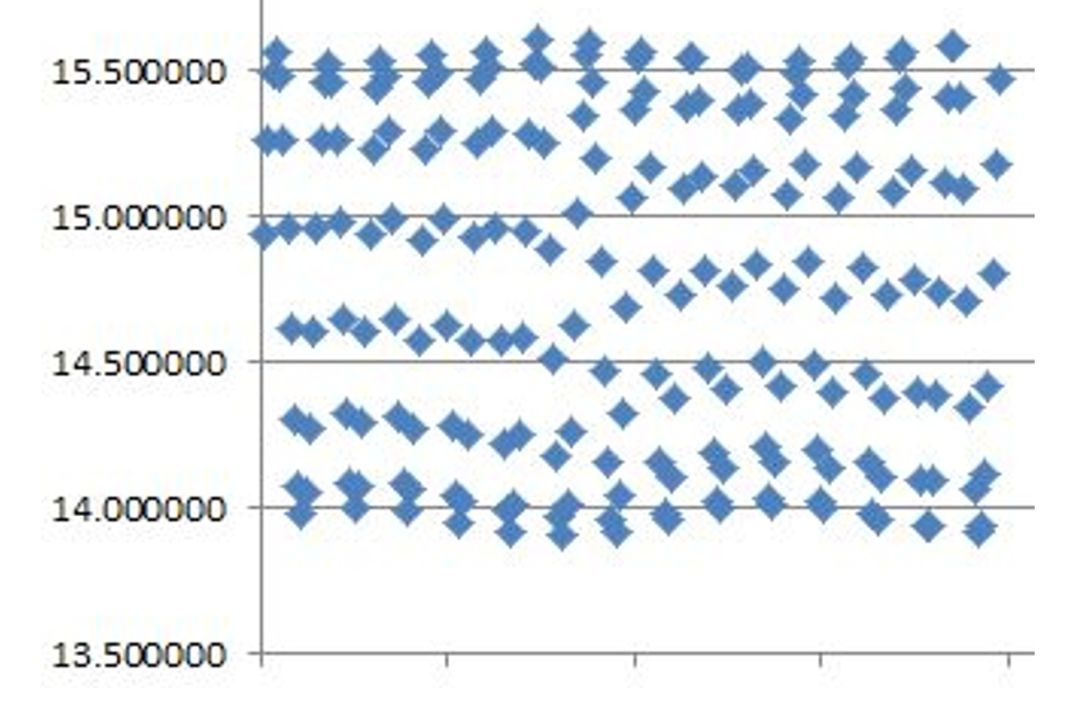
\includegraphics[width=0.5\linewidth]{IMG/201910/191009.jpeg}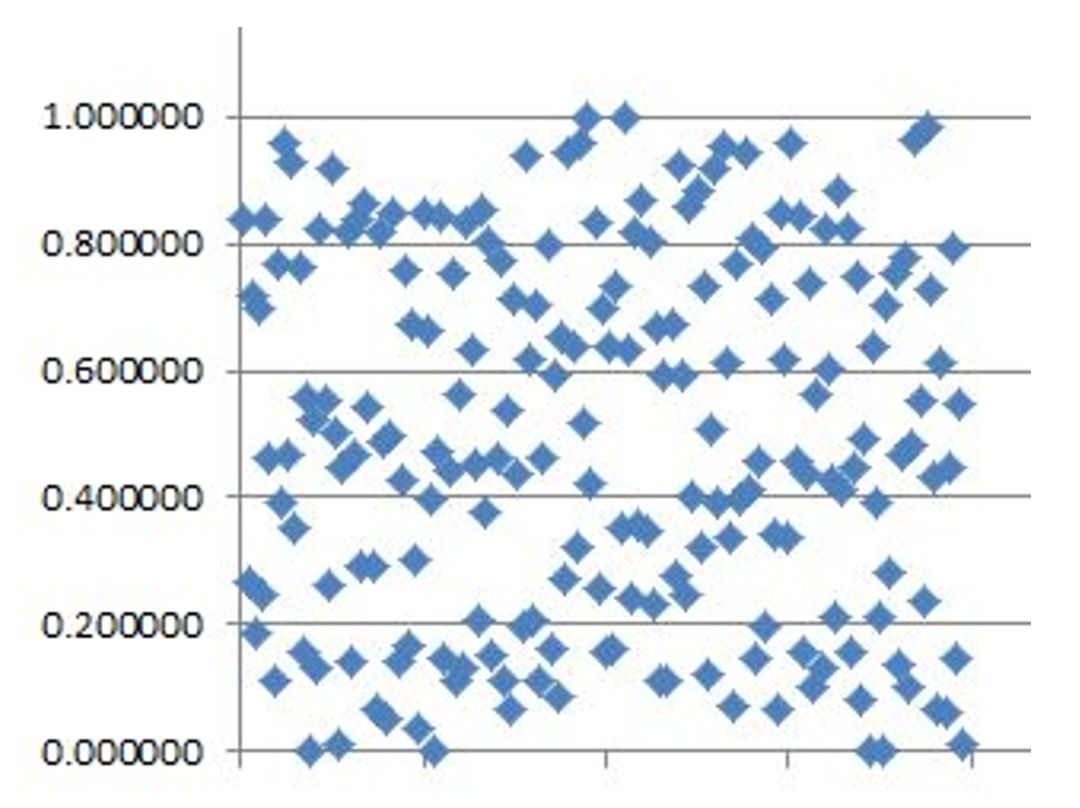
\includegraphics[width=0.5\linewidth]{IMG/201910/191010.jpeg}
 
发现朔月的分布时间在24小时内几乎平均分布,其平均值约为0.49天. 

据此我们计算出平均满月的出现时间为:满月时间(平均)=朔月时间(平均)+朔望月时间差(平均),得到平均出现望月的时间为15.26天,大于15天,由于计算的满月时间为天数差值,从第一天算还得加上一天,据此得到“十五的月亮十六圆”!


\noindent\qiangdiao{Q2为什么集装箱的表面都是凹凸不平的?}

这种凹凸结构在工程上称为槽形舱壁,槽形舱壁的剖面形状如图所示,有三角形、矩形、梯形、弧形等,其中,以梯形剖面应用较广. 

\noindent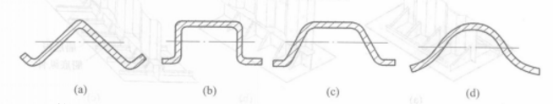
\includegraphics[width=\linewidth]{IMG/201910/191012.png}

槽形舱壁由钢板压制而成,以它的槽形折曲来代替扶强材(\textit{为保证金属板的刚性所加装的钢质船体结构材料})的作用. 槽形舱壁与平面舱壁相比较,其优点是在保证同样的强度条件下,可以减轻结构重量,节省钢材. 同时,也减少了装配和焊接的工作量. 在散货船和油船上,更便于清舱,有利防止锈蚀. 但槽形舱壁也存在缺点,主要是它在垂直于槽形方向的承压能力较差;此外,若要保证槽形舱壁的强度,就必须使槽形体具有一定的深度,占据较大舱容,对于杂货船的舱容没有利,但对散货船和油船无影响. 所以,槽形舱壁用于散货船和油船居多. 

\noindent\qiangdiao{Q3为什么行星运动的轨道都是椭圆的?}

“所有行星绕太阳的轨道都是椭圆,太阳在椭圆的一个焦点上”开普勒第一定律告诉我们围绕太阳运动的行星沿椭圆轨道运行. 后期学者将开普勒第一定律修改为更为普适的:所有行星和彗星的轨道都属圆锥曲线,而太阳则在它们的一个焦点上. 

在万有引力的作用下,求解极坐标系下的径向运动方程可以得到行星的运动轨迹为圆锥曲线:
\[
\frac{1}{r}=\frac{GMm^2}{l^2}(1+e\cos\theta), e=\frac{Cl^2}{GMm^2}.
\]

$e$是离心率. 当$0<e<1$时,对应的轨道即为椭圆轨道,对于太阳系中具有稳定周期的行星而言,其轨道均为椭圆轨道. 当$e=1$时为抛物线轨道,$e>1$时为双曲线轨道,这两种都对应于非周期彗星,这些彗星一生中只能接近太阳一次. 

综上,只考虑太阳对行星的万有引力作用,太阳系中稳定存在的行星轨道都为椭圆. 


\noindent\qiangdiao{Q4为什么功率较小的电风扇,在把插头拔掉后重新按开关还能转1到2圈?是因为具有惯性吗?}

小功率风扇通常指带USB接口的风扇. 这种风扇在使用的时候一般需要搭配一个起变压作用的充电头,由于这种充电头包含可变压的元件,这些元件会起到电感,电容的作用. 在正常通电工作时,电感会将一部分能量储存在磁场中,而电容会把能量储存在电场中. 断电时,原本储存在磁场和电场中的能量会重新输入到电路中. 因此即便已经断电了,但是电路中的能量并没有马上消失. 这时重新按开关的话,风扇还能重新转几圈. 而直接用220V电压供电的风扇就不会出现这种现象. 

\end{multicols}

\ADhairui

